\section{Обзор предметной области}
\label{sec:domain}

В данном разделе будет произведён обзор предметной области задачи, решаемой в рамках дипломной работы; рассмотрены вопросы о сущности нейронных сетей и принципе их работ.

\subsection{Нейронные сети}
\label{sub:domain:neuro_net}
Нейронные сети – это одно из направлений исследований в области искусственного интеллекта, основанное на попытках воспроизвести нервную систему человека, а именно: способность нервной системы обучаться и исправлять ошибки, что должно позволить смоделировать, хотя и достаточно грубо, работу человеческого мозга~\cite{domain_aiportal}.

Биологический нейрон – это специальная клетка, которая структурно состоит из ядра, тела клетки и отростков.
Одной из ключевых задач нейрона является передача электрохимического импульса по всей нейронной сети через доступные связи с другими нейронами.
Притом, каждая связь характеризуется некоторой величиной, называемой силой синаптической связи.
Эта величина определяет, что произойдет с электрохимическим импульсом при передаче его другому нейрону: либо он усилится, либо он ослабится, либо останется неизменным.

Биологическая нейронная сеть обладает высокой степенью связности: на один нейрон может приходиться несколько тысяч связей с другими нейронами.
Но, это приблизительное значение и в каждом конкретном случае оно разное.
Передача импульсов от одного нейрона к другому порождает определенное возбуждение всей нейронной сети.
Величина этого возбуждения определяет реакцию нейронной сети на какие-то входные сигналы.
Например, встреча человека со старым знакомым может привести к сильному возбуждению нейронной сети, если с этим знакомым связаны какие-то яркие и приятные жизненные воспоминания.
В свою очередь сильное возбуждение нейронной сети может привести к учащению сердцебиения, более частому морганию глаз и к другим реакциям.
Встреча же с незнакомым человеком для нейронной сети пройдет практически незаметной, а значит и не вызовет каких-либо сильных реакций.

Искусственная нейронная сеть представляет из себя математическую модель, построенную по принципу организации и функционирования биологических нейронных сетей.
Сеть состоит из системы соединенных и взаимодействующих между собой простых процессоров.
Эти процессоры обрабатывают входные сигналы и передает остальным.
Обычно сложных операций они не производят, однако соединенные в большую сеть, могут выполнять сложные задачи.

Каждый нейрон выполняет небольшой объем работ --- например, суммирует пришедшие на него сигналы с некоторыми весовыми коэффициентами и дополнительно нелинейно преобразует эту взвешенную сумму входных данных.
Другим распространённым вариантом является нейрон-детектор, выдающий высокий выходной сигнал при малых отличиях своих входных сигналов от некоторого запомненного эталона, и низкий выходной сигнал при существенных отличиях.

Нейроны группируются в последовательность слоёв; входные сигналы поступают на первый слой и последовательно проходят через все слои до последнего, выходного слоя сети.
Но бывают и рекуррентные структуры, обеспечивающие циркуляцию некоторого набора внутренних сигналов.

Нейроны, составляющие некоторый слой сети, работают в параллельном режиме.
Изменение числа слоёв и количества нейронов в слоях позволяет гибко или максимально эффективно настроить общий параллельно-последовательный объем вычислений на особенности применяемой вычислительной техники.

Процесс работы с сетью представляет собой движение потока внешних сенсорных данных от входных нейронов к выходным и преобразование этих данных.
В общем случае поток сигналов может формировать и перекрёстные, и обратные связи~\cite{domain_neuropro}.

Нейронная сеть способна обучаться решению задач, для которых у человека не существует формализованных, быстрых или работающих с приемлемой точностью теоретических или эмпирических алгоритмов.
Наряду с обучающими данными требуется лишь задать некоторый критерий качества решения задачи, который нейронная сеть при своём обучении должна будет минимизировать или оптимизировать.

Структура сети может быть адаптирована к задаче.
В сеть могут быть включены дополнительные нейроны и даже слои нейронов, если исходно она была не способна обеспечить нужную точность решения.
Из нейронной сети могут быть исключены лишние нейроны и связи между ними, если исходная сеть была избыточна.
Cеть может сама выделить наиболее информативные для задачи входные сигналы, отбросить неинформативные, шумовые сигналы и в итоге повысить надежность решения.
При этом коррекция размеров нейронной сети не приводит к полному забыванию ранее сформированных при обучении навыков, что ускоряет последующий процесс обучения~\cite{domain_neuropro}.

Нейронные сети не программируются в привычном смысле этого слова, они обучаются.
Возможность обучения — одно из главных преимуществ нейронных сетей перед традиционными алгоритмами.
Технически обучение заключается в нахождении коэффициентов связей между нейронами.
В процессе обучения нейронная сеть способна выявлять сложные зависимости между входными данными и выходными, а также выполнять обобщение. Это значит, что в случае успешного обучения сеть сможет вернуть верный результат на основании данных, которые отсутствовали в обучающей выборке, а также неполных и повреждённых, частично искаженных данных.

\subsection{Типы нейронных сетей}
\label{sub:domain:neuro_net_types}

Существует несколько типов нейронных сетей: многослойный перцептрон, рекуррентный перцептрон, ассоциативная память, сверточные нейронные сети, сети Кохонена и спайковые сети.

Многослойный перцептрон самая известная и архитектура, в которой идут подряд несколько слоев нейронов --- входной, один или несколько скрытых слоев, и выходной слой.
Почти всегда обучается методом обратного распространения ошибки --- что автоматически означает, что мы должны предоставить для обучения набор пар «входной вектор --- правильный выход»\cite{domain_romanov}.
Тогда входной вектор отправится на вход сети, последовательно будут рассчитаны состояния всех промежуточных нейронов, и на выходе образуется выходной вектор, который мы и сравним с правильным.
Расхождение даст нам ошибку, которую можно распространить обратно по связям сети, вычислить вклад в итоговую ошибку каждого нейрона, и скорректировать его веса, чтобы ее исправить.
Повторив эту процедуру много тысяч раз, возможно выйдет обучить сеть.

Сеть такого типа очень хорошо справляется с задачами, где ответ действительно зависит только от того, что мы даем на вход сети, и никак не зависит от истории входов (т.е. это не последовательность информации со скрытой закономерностью; ответ не зависит или слабо зависит от высоких степеней или произведений параметров --- функции этого типа сеть строить почти не умеет; в наличии есть достаточно много примеров (желательно иметь не менее сотни примеров на каждую связь сети), или у вас есть большой опыт борьбы с эффектом специализации.
Это связано с тем, что имея много коэффициентов, сеть может банально запомнить много конкретных примеров, и выдавать на них отличный результат --- но ее прогнозы не будут иметь ничего общего с реальностью в случае, если дать на вход примеры не из обучающей выборки.

Слабые стороны --- неумение работать с динамическими процессами, необходимость большой обучающей выборки.
Рекуррентный перцептрон на первый взгляд поход на обычный перцептрон, единственное существенное отличие состоит в том, что его выходные сигналы попадают ему же на входы, и участвуют в обработке уже следующего входного вектора сигналов.

То есть, в случае рекуррентного перцептрона имеет место не набор отдельных, ничем не связанных образов, а некоторый процесс, и значение имеют не только сами входы, но и то, в какой последовательности они поступают.
Из-за этого возникают отличия в методе обучения --- используется то же самое обратное распространение ошибки, но для того, чтобы ошибка попала по рекуррентной связи в прошлое, используются разные ухищрения.
В остальном же ситуация похожа на обычный перцептрон --- для обучения нужно иметь достаточно длинную последовательность пар вход-выход, которую нужно много раз прогнать через сеть, чтобы ее обучить или же иметь под рукой математическую модель искомого процесса, которую можно гонять во всевозможных условиях, и в режиме реального времени давать результаты сети для обучения.
Сеть такого типа обычно хорошо решает задачи управления динамическими процессами начиная от классической задачи стабилизации перевернутого маятника, и до любых систем, которыми вообще хоть как-то получается управлять, предсказания динамических процессов, и вообще всего, где помимо явно наблюдаемого входа у системы есть некоторое внутреннее состояние, которое не совсем понятно, как использовать.

Ассоциативная память --- это широкий класс сетей, которые в той или иной степени напоминают архитектуру Хопфилда, которая состоит из одного слоя нейронов, выходы которого поступают на его входы в следующий момент времени.
Этот слой служит и входом сети.
В начальный момент выходы нейронов принимаются равными входному вектору, и ее выходом --- значения на нейронах, образовавшиеся в конце работы, считаются ответом сети.
Данный тип сетей меняет свои состояния с течением времени до тех пор, пока состояние не перестанет меняться.
Свойства весовой матрицы выбраны таким образом, чтобы устойчивое состояние всегда гарантированно достигалось и обычно это происходит за несколько шагов.
Такая сеть помнит некоторое количество векторов, и при подаче на вход любого вектора, может определить, на какой из запомненных он более всего похож --- отсюда и название~\cite{domain_neuro_tech}.

Двухслойная модификация этой сети, а именно гетероассоциативная память, может запоминать вектора не по одному, а по парам разной размерности.
Сети такого типа хорошо справляются с задачами, где нужно определить похожесть вектора на один из стандартных запомненных.
Собственно, это единственный класс задач, где они хороши.
Также конкретно сеть Хопфилда может использоваться для решения задач оптимизации, например, задачи коммивояжёра, однако ее эффективность в этой области под вопросом.
К сильным сторонам можно отнести --- очень быстрое обучение, возможность удалить образ из памяти или добавить в память, не затронув остальные, некоторые свойства такой памяти напоминают свойства мозга, и их изучение интересно с такой позиции~\cite{domain_neuro_tech}.
Слабые стороны --- очень узкий класс решаемых задач, неумение обобщать примеры, максимальный объем памяти жестко связан с размерностью запоминаемого вектора, ввиду особенностей построения.
Перспективы:

\begin{itemize}
  \item разработана ядерная ассоциативная память, которая способна к обобщению образов, и имеет неограниченный объем памяти, потому что сеть растет по мере заполнения;
  \item разработана динамическая ассоциативная память, которая запоминает не отдельные образы, а определенные последовательности образов, и поэтому может применяться для распознавания элементов динамических процессов;
  \item динамическая ассоциативная память демонстрирует способность к генерации отклика, содержащего разные элементы запомненных последовательностей при подаче входного сигнала, соответствующего одновременно разным последовательностям, что, возможно, является некоторой грубой моделью творчества человека;
  \item гибрид ядерной и динамической ассоциативной памяти может дать новое качество в распознавании последовательностей — например, в распознавании речи.
\end{itemize}

Нейронные сети Кохонена --- класс нейронных сетей, основным элементом которых является слой Кохонена.
Слой Кохонена состоит из адаптивных линейных сумматоров.
Как правило, выходные сигналы слоя обрабатываются по правилу «победитель получает всё»: наибольший сигнал превращается в единичный, остальные обращаются в ноль~\cite{domain_kohonen}.

По способам настройки входных весов сумматоров и по решаемым задачам различают много разновидностей сетей Кохонена.
Наиболее известные из них:
\begin{itemize}
  \item сети векторного квантования сигналов, тесно связанные с простейшим базовым алгоритмом кластерного анализа (метод динамических ядер или K-средних);
  \item самоорганизующиеся карты Кохонена;
  \item сети векторного квантования, обучаемые с учителем.
\end{itemize}

Самоорганизующаяся карта Кохонена --- нейронная сеть с обучением без учителя, выполняющая задачу визуализации и кластеризации.
Идея сети предложена финским учёным Т. Кохоненом.
Является методом проецирования многомерного пространства в пространство с более низкой размерностью (чаще всего, двумерное), применяется также для решения задач моделирования, прогнозирования и др.
Является одной из версий нейронных сетей Кохонена.
Самоорганизующиеся карты Кохонена используются для решения таких задач, как моделирование, прогнозирование, выявление наборов независимых признаков, сжатие информации, а также для поиска закономерностей в больших массивах данных.
Наиболее часто описываемый алгоритм применяется для кластеризации данных.

Самоорганизующаяся карта состоит из компонентов, называемых узлами или нейронами.
Их количество задаётся аналитиком. Каждый из узлов описывается двумя векторами.
Первый --- т. н. вектор веса m, имеющий такую же размерность, что и входные данные.
Второй --- вектор r, представляющий собой координаты узла на карте.
Карта Кохонена визуально отображается с помощью ячеек прямоугольной или шестиугольной формы;
последняя применяется чаще, поскольку в этом случае расстояния между центрами смежных ячеек одинаковы, что повышает корректность визуализации карты~\cite{domain_kohonen}.

Изначально известна размерность входных данных, по ней некоторым образом строится первоначальный вариант карты.
В процессе обучения векторы веса узлов приближаются к входным данным.
Для каждого наблюдения выбирается наиболее похожий по вектору веса узел, и значение его вектора веса приближается к наблюдению.
Также к наблюдению приближаются векторы веса нескольких узлов, расположенных рядом, таким образом если в множестве входных данных два наблюдения были схожи, на карте им будут соответствовать близкие узлы.
Циклический процесс обучения, перебирающий входные данные, заканчивается по достижении картой допустимой (заранее заданной аналитиком) погрешности, или по совершении заданного количества итераций.
Таким образом, в результате обучения карта Кохонена классифицирует входные данные на кластеры и визуально отображает многомерные входные данные в двумерной плоскости, распределяя векторы близких признаков в соседние ячейки и раскрашивая их в зависимости от анализируемых параметров нейронов.
В результате работы алгоритма получаются следующие карты: карта входов нейронов --- визуализирует внутреннюю структуру входных данных путем подстройки весов нейронов карты.
Обычно используется несколько карт входов, каждая из которых отображает один из них и раскрашивается в зависимости от веса нейрона~\cite{domain_kohonen}.
На одной из карт определенным цветом обозначают область, в которую включаются приблизительно одинаковые входы для анализируемых примеров; карта выходов нейронов --- визуализирует модель взаимного расположения входных примеров.

Очерченные области на карте представляют собой кластеры, состоящие из нейронов со схожими значениями выходов.
Cпециальные карты — это карта кластеров, полученных в результате применения алгоритма самоорганизующейся карты Кохонена, а также другие карты, которые их характеризуют.

\subsection{Многослойные перцептроны}
\label{sub:domain:perceptrons}

Многослойными персептронами называют нейронные сети прямого распространения.
Входной сигнал в таких сетях распространяется в прямом направлении, от слоя к слою.
Многослойный персептрон в общем представлении состоит из следующих элементов:

\begin{itemize}
  \item множества входных узлов, которые образуют входной слой;
  \item одного или нескольких скрытых слоев вычислительных нейронов;
  \item одного выходного слоя нейронов.
\end{itemize}

Искуусственный нейрон --- узел искусственной нейронной сети, являющийся упрощённой моделью естественного нейрона. Математически, искусственный нейрон обычно представляют как некоторую нелинейную функцию от единственного аргумента --- линейной комбинации всех входных сигналов. Данную функцию называют функцией активации. Полученный результат посылается на единственный выход. Такие искусственные нейроны объединяют в сети --- соединяют выходы одних нейронов с входами других. Искусственные нейроны и сети являются основными элементами идеального нейрокомпьютера
Многослойный персептрон представляет собой обобщение однослойного персептрона Розенблатта~\cite{domain_rosenblatt}.

\begin{figure}[ht]
\centering
  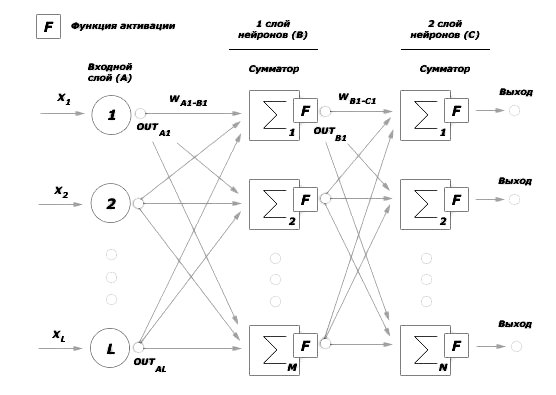
\includegraphics[scale=1]{domain_perceptron_scheme.jpg}
  \caption{ Схема двухслойного перцептрона }
  \label{fig:perceptron_scheme}
\end{figure}

Примером многослойного персептрона является следующая модель нейронной сети(рисунок~\ref{fig:perceptron_scheme}).

Многослойные персептроны успешно применяются для решения разнообразных сложных задач и имеют следующих три отличительных признака.

Свойство 1. Каждый нейрон сети имеет нелинейную функцию активации

Важно подчеркнуть, что такая нелинейная функция должна быть гладкой (т.е. всюду дифференцируемой), в отличие от жесткой пороговой функции, используемой в персептроне Розенблатта.
Самой популярной формой функции, удовлетворяющей этому требованию, является сигмоидальная. Примером сигмоидальной функции может служить логистическая функция, задаваемая следующим выражением:

\begin{equation}
  \label{eq:domain:activation_function}
  f(x)=\frac{2}{1+e^{ax}}-1
\end{equation}
\begin{explanation}
  где & $ a $ & параметр наклона сигмоидальной функции. Изменяя этот параметр, можно построить функции с различной крутизной.
\end{explanation}

Наличие нелинейности играет очень важную роль(рисунок~\ref{fig:perceptron_scheme}), так как в противном случае отображение «вход-выход» сети можно свести к обычному однослойному персептрону
Монотонно возрастающая всюду дифференцируемая S-образная нелинейная функция с насыщением. Сигмоид позволяет усиливать слабые сигналы и не насыщаться от сильных сигналов. Гроссберг (1973 год) обнаружил, что подобная нелинейная функция активации решает поставленную им дилемму шумового насыщения.
Слабые сигналы нуждаются в большом сетевом усилении, чтобы дать пригодный к использованию выходной сигнал. Однако усилительные каскады с большими коэффициентами усиления могут привести к насыщению выхода шумами усилителей, которые присутствуют в любой физически реализованной сети. Сильные входные сигналы в свою очередь также будут приводить к насыщению усилительных каскадов, исключая возможность полезного использования выхода. Таким образом одна и та же сеть может обрабатывать как слабые, так и сильные сигналы.

\begin{figure}[ht]
\centering
  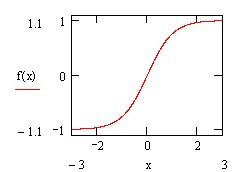
\includegraphics[scale=1]{domain_bipolar_sigmoidal_function.jpg}
  \caption{ Биполярная сигмоидальная функция }
  \label{fig:bipolar_sigmoidal_function}
\end{figure}

Свойство 2. Несколько скрытых слоев

Многослойный персептрон содержит один или несколько слоев скрытых нейронов, не являющихся частью входа или выхода сети.
Эти нейроны позволяют сети обучаться решению сложных задач, последовательно извлекая наиболее важные признаки из входного образа.

Свойство 3. Высокая связность

Многослойный персептрон обладает высокой степенью связности, реализуемой посредством синаптических соединений.
Изменение уровня связности сети требует изменения множества синаптических соединений или их весовых коэффициентов.

Комбинация всех этих свойств наряду со способностью к обучению на собственном опыте обеспечивает вычислительную мощность многослойного персептрона~\cite{domain_rosenblatt}.
Однако эти же качества являются причиной неполноты современных знаний о поведении такого рода сетей: распределенная форма нелинейности и высокая связность сети существенно усложняют теоретический анализ многослойного персептрона.
